% Drawing 154/09-1 -- folder 154, batch 09, archive page 161 (PDF page 162).
% Transcription: page de dessins sans texte suivi. En haut à gauche, au crayon, un disque traversé de trois pseudo-droites rouges qui se croisent près du centre, l'une dessinant une boucle étroite. En haut au milieu, un disque traversé de pseudo-droites rouges, plusieurs triangles coloriés en jaune, le bord doublé de tirets vert foncé et vert clair ; au bord, de petits numéros, en partie lisibles ($1$, $1'$, $2'$, $4'$, $5$). Au centre, un disque à bord rouge partagé par des arcs vert clair et vert foncé entre deux points $a$ (en bas) et $b$ (en haut), numéros $1$ à $5$ et $1'$ à $5'$ le long des arcs ; deux flèches en partent vers deux copies du même disque, les arcs doublés de pointillés et de tirets rouges, puis vers deux demi-disques, l'un fléché vers le haut le long des numéros $5'$, $4'$, $3'$, $2'$, l'autre vers le bas le long de $2$, $3$, $4$, $5$. En bas à gauche, au crayon, deux cercles superposés, l'arc supérieur $\alpha$ de $a$ à $b$, l'arc inférieur $\beta$ de $b$ à $a$, fléchés, avec deux orientations marquées $\omega$ ; à côté, un demi-disque dont le diamètre porte $\alpha$ au-dessus et $\beta$ au-dessous. En bas à droite, un rectangle bordé de rouge rempli d'arcs orange entrelacés, et un rectangle rouge coupé en deux par une bande vert clair
% Kind: page of drawings: pencil disk with three pseudolines; disk with red arrangement and yellow triangles; small disks with green arcs; half-disks; rectangles. Method 2 (schematic redraw from the facsimile). Status: partial.
% Notes: Page of drawings without running text, read from the page view. Top left, in pencil, a disk crossed by three red pseudolines crossing near the centre, one making a narrow loop. Top middle, a disk crossed by red pseudolines, several triangles coloured yellow, rims dashed in green and yellow, numbered points (not reproduced). Middle: a small disk divided by red and green arcs between b and a, arrows to two further disks with green arcs (dotted red rims) and to half-disks with dotted rims and small numbered strokes. Below: pencil figures (a figure eight with arrows a, b, alpha, beta), a red rectangle filled with orange arcs and a red rectangle divided in three bands. Strands schematic.
% Coordinates: 1 unit = 1 mm = 1/100 of the crop width (bbox in page fractions: [0.175, 0.085, 0.864, 0.502]).
% Redrawn by Claude (claude-opus-5-5), issue #73, 2026-11-07; not checked by a human; not compiled (no TeX in the session).
% Rights: reproduces part of the work -- behind RENDER_TRANSCRIPTS, never published by itself.
\documentclass[tikz,border=3pt]{standalone}
\usepackage{amsmath,amssymb}
\usetikzlibrary{patterns,arrows.meta}
\tikzset{Or/.style={orange!90!black}, Ye/.style={yellow!80!orange}, Lg/.style={green!60!black!70}, Dg/.style={green!45!black}, Br/.style={brown!80!black}, Rd/.style={red!85!black}, Bl/.style={blue!70!black}, Gy/.style={black!40}, pencil/.style={black!45}, struck/.style={black!35}, mark/.style={circle,draw,inner sep=1.3pt}, pt/.style={circle,fill,inner sep=0.9pt}, opt/.style={circle,draw,fill=white,inner sep=1.1pt}}
\begin{document}
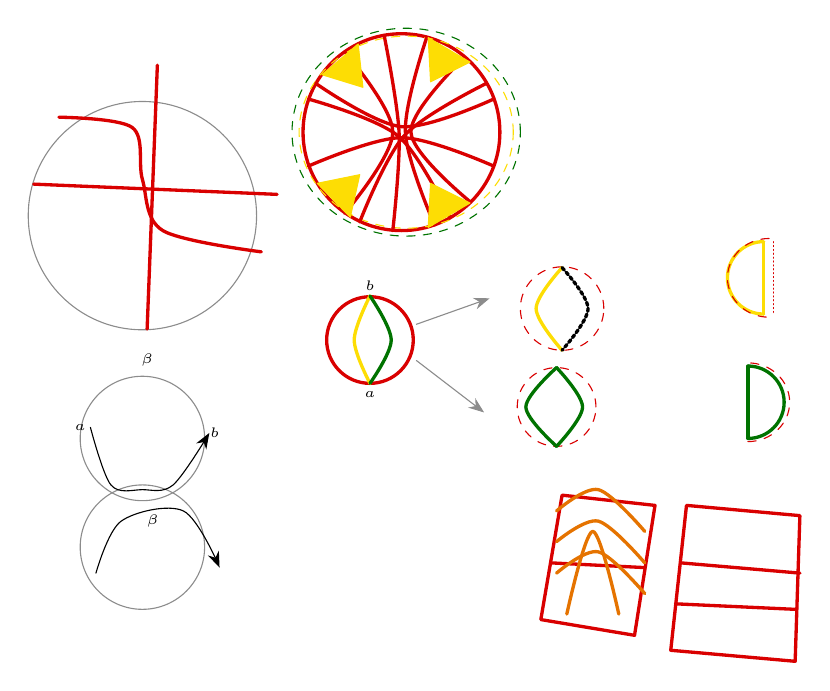
\begin{tikzpicture}[x=1mm,y=1mm,line cap=round,line join=round,font=\scriptsize]
\draw[pencil] (14.5,-27) circle[radius=14.5];
\draw[Rd,very thick] (0.7,-23) -- (31.6,-24.3);
\draw[Rd,very thick] (16.4,-7.9) -- (15.1,-41.4);
\draw[Rd,very thick] plot[smooth, tension=0.55] coordinates {(3.9,-14.5) (13.2,-15.8) (14.5,-22.4) (17.1,-28.9) (29.6,-31.6)};
\draw[Rd,very thick] (47.4,-16.4) circle[radius=12.5];
\draw[Dg,dashed] (48,-16.4) ellipse[x radius=14.5, y radius=13.2];
\draw[Ye,dashed] (48,-16.4) ellipse[x radius=13.6, y radius=12.2];
\draw[Rd,very thick] plot[smooth, tension=0.55] coordinates {(45.2,-4.1) (47.1,-16.5) (46.3,-28.9)};
\draw[Rd,very thick] plot[smooth, tension=0.55] coordinates {(50.6,-4.4) (47.9,-16.4) (51.6,-28.2)};
\draw[Rd,very thick] plot[smooth, tension=0.55] coordinates {(40.2,-6.2) (46.3,-16.4) (40.2,-26.7)};
\draw[Rd,very thick] plot[smooth, tension=0.55] coordinates {(55.4,-6.9) (48.6,-16.4) (56.2,-25.3)};
\draw[Rd,very thick] plot[smooth, tension=0.55] coordinates {(36.5,-10.2) (47.4,-15.7) (59.1,-12.2)};
\draw[Rd,very thick] plot[smooth, tension=0.55] coordinates {(35.6,-20.7) (47.4,-17.1) (59.1,-20.7)};
\draw[Rd,very thick] plot[smooth, tension=0.55] coordinates {(58.2,-10.2) (47.8,-16.8) (42.1,-27.8)};
\draw[Rd,very thick] plot[smooth, tension=0.55] coordinates {(35.6,-12.2) (47,-16.9) (53.6,-27.3)};
\draw[Ye] (41.9,-5.2) -- (37.3,-9.1) -- (42.5,-10.7) -- cycle;
\fill[pattern=north east lines,Ye] (41.9,-5.2) -- (37.3,-9.1) -- (42.5,-10.7) -- cycle;
\draw[Ye] (56.1,-7.5) -- (50.8,-4.4) -- (51.1,-10) -- cycle;
\fill[pattern=north east lines,Ye] (56.1,-7.5) -- (50.8,-4.4) -- (51.1,-10) -- cycle;
\draw[Ye] (36.7,-22.9) -- (40.9,-27.2) -- (42.1,-21.8) -- cycle;
\fill[pattern=north east lines,Ye] (36.7,-22.9) -- (40.9,-27.2) -- (42.1,-21.8) -- cycle;
\draw[Ye] (50.8,-28.5) -- (56.1,-25.4) -- (51.1,-22.9) -- cycle;
\fill[pattern=north east lines,Ye] (50.8,-28.5) -- (56.1,-25.4) -- (51.1,-22.9) -- cycle;
\draw[Rd,very thick] (43.4,-42.8) circle[radius=5.5];
\draw[Ye,very thick] plot[smooth, tension=0.55] coordinates {(43.4,-37.2) (41.4,-42.8) (43.4,-48.3)};
\draw[Dg,very thick] plot[smooth, tension=0.55] coordinates {(43.4,-37.2) (46.1,-42.8) (43.4,-48.3)};
\node[inner sep=1pt] at (43.4,-35.9) {\tiny $b$};
\node[inner sep=1pt] at (43.4,-49.7) {\tiny $a$};
\draw[-{Stealth[length=2mm]},pencil] (49.3,-40.8) -- (58.6,-37.5);
\draw[-{Stealth[length=2mm]},pencil] (49.3,-45.4) -- (57.9,-52);
\draw[Rd,dashed] (67.8,-38.8) circle[radius=5.3];
\draw[Ye,very thick] plot[smooth, tension=0.55] coordinates {(67.8,-33.6) (64.5,-38.8) (67.8,-44.1)};
\draw[very thick,densely dotted] plot[smooth, tension=0.55] coordinates {(67.8,-33.6) (71.1,-38.8) (67.8,-44.1)};
\draw[Rd,dashed] (67.1,-51.3) circle[radius=5];
\draw[Dg,very thick] plot[smooth, tension=0.55] coordinates {(67.1,-46.3) (63.2,-51.3) (67.1,-56.3)};
\draw[Dg,very thick] plot[smooth, tension=0.55] coordinates {(67.1,-46.3) (70.4,-51.3) (67.1,-56.3)};
\draw[Ye,very thick] (93.4,-30.3) arc[start angle=90, end angle=270, x radius=4.6, y radius=4.6];
\draw[Ye,very thick] (93.4,-30.3) -- (93.4,-39.5);
\draw[Rd,dashed] (94.1,-29.9) arc[start angle=90, end angle=270, x radius=5.3, y radius=5];
\draw[Rd,densely dotted] (94.7,-30.3) -- (94.7,-39.5);
\draw[Dg,very thick] (91.4,-55.3) arc[start angle=-90, end angle=90, x radius=4.6, y radius=4.6];
\draw[Dg,very thick] (91.4,-46.1) -- (91.4,-55.3);
\draw[Rd,dashed] (91.4,-55.7) arc[start angle=-90, end angle=90, x radius=5.3, y radius=5];
\draw[pencil] (14.5,-55.3) circle[radius=7.9];
\draw[pencil] (14.5,-69.1) circle[radius=7.9];
\draw[-{Stealth[length=2mm]}] plot[smooth, tension=0.55] coordinates {(7.9,-53.9) (10.5,-61.2) (14.5,-61.8) (18.4,-61.2) (23,-54.6)};
\draw[-{Stealth[length=2mm]}] plot[smooth, tension=0.55] coordinates {(8.6,-72.4) (11.8,-65.8) (19.7,-64.5) (24.3,-71.7)};
\node[inner sep=1pt] at (6.6,-53.9) {\tiny $a$};
\node[inner sep=1pt] at (23.7,-54.6) {\tiny $b$};
\node[inner sep=1pt] at (15.1,-45.4) {\tiny $\beta$};
\node[inner sep=1pt] at (15.8,-65.8) {\tiny $\beta$};
\draw[Rd,very thick] (67.8,-62.5) -- (79.6,-63.8) -- (77,-80.3) -- (65.1,-78.3) -- cycle;
\draw[Rd,very thick] (66.4,-71.1) -- (78.3,-71.7);
\draw[Or,very thick] plot[smooth, tension=0.55] coordinates {(67.1,-64.5) (72.4,-61.8) (78.3,-67.1)};
\draw[Or,very thick] plot[smooth, tension=0.55] coordinates {(67.1,-68.4) (72.4,-65.8) (78.3,-71.1)};
\draw[Or,very thick] plot[smooth, tension=0.55] coordinates {(67.1,-72.4) (72.4,-69.7) (78.3,-75)};
\draw[Or,very thick] plot[smooth, tension=0.55] coordinates {(68.4,-77.6) (71.7,-67.1) (75,-77.6)};
\draw[Rd,very thick] (83.6,-63.8) -- (98,-65.1) -- (97.4,-83.6) -- (81.6,-82.2) -- cycle;
\draw[Rd,very thick] (82.9,-71.1) -- (98,-72.4);
\draw[Rd,very thick] (82.2,-76.3) -- (97.4,-77);
\end{tikzpicture}
\end{document}
